% Options for packages loaded elsewhere
\PassOptionsToPackage{unicode}{hyperref}
\PassOptionsToPackage{hyphens}{url}
%
\documentclass[
  14pt,
]{extarticle}
\usepackage{lmodern}
\usepackage{amssymb,amsmath}
\usepackage{ifxetex,ifluatex}
\ifnum 0\ifxetex 1\fi\ifluatex 1\fi=0 % if pdftex
  \usepackage[T1]{fontenc}
  \usepackage[utf8]{inputenc}
  \usepackage{textcomp} % provide euro and other symbols
\else % if luatex or xetex
  \usepackage{unicode-math}
  \defaultfontfeatures{Scale=MatchLowercase}
  \defaultfontfeatures[\rmfamily]{Ligatures=TeX,Scale=1}
\fi
% Use upquote if available, for straight quotes in verbatim environments
\IfFileExists{upquote.sty}{\usepackage{upquote}}{}
\IfFileExists{microtype.sty}{% use microtype if available
  \usepackage[]{microtype}
  \UseMicrotypeSet[protrusion]{basicmath} % disable protrusion for tt fonts
}{}
\makeatletter
\@ifundefined{KOMAClassName}{% if non-KOMA class
  \IfFileExists{parskip.sty}{%
    \usepackage{parskip}
  }{% else
    \setlength{\parindent}{0pt}
    \setlength{\parskip}{6pt plus 2pt minus 1pt}}
}{% if KOMA class
  \KOMAoptions{parskip=half}}
\makeatother
\usepackage{xcolor}
\IfFileExists{xurl.sty}{\usepackage{xurl}}{} % add URL line breaks if available
\IfFileExists{bookmark.sty}{\usepackage{bookmark}}{\usepackage{hyperref}}
\hypersetup{
  hidelinks,
  pdfcreator={LaTeX via pandoc}}
\urlstyle{same} % disable monospaced font for URLs
\usepackage{graphicx}
\makeatletter
\def\maxwidth{\ifdim\Gin@nat@width>\linewidth\linewidth\else\Gin@nat@width\fi}
\def\maxheight{\ifdim\Gin@nat@height>\textheight\textheight\else\Gin@nat@height\fi}
\makeatother
% Scale images if necessary, so that they will not overflow the page
% margins by default, and it is still possible to overwrite the defaults
% using explicit options in \includegraphics[width, height, ...]{}
\setkeys{Gin}{width=\maxwidth,height=\maxheight,keepaspectratio}
% Set default figure placement to htbp
\makeatletter
\def\fps@figure{htbp}
\makeatother
\setlength{\emergencystretch}{3em} % prevent overfull lines
\providecommand{\tightlist}{%
  \setlength{\itemsep}{0pt}\setlength{\parskip}{0pt}}
\setcounter{secnumdepth}{-\maxdimen} % remove section numbering
\ifluatex
  \usepackage{selnolig}  % disable illegal ligatures
\fi

\author{}
\date{}

\begin{document}

\hypertarget{optimal-margins}{%
\section{Optimal Margins}\label{optimal-margins}}

\hypertarget{the-general-case}{%
\subsection{The General Case}\label{the-general-case}}

\begin{itemize}
\tightlist
\item
  Given an \(N\times k\) feature matrix \(X\) in ``tidy'' format as
  usual.
\item
  We also have an \(N\times 1\) vector \(Y\) whose entries are
  \(\pm 1\). \(Y\) distinguishes the two classes in the data.
\item
  The goal is to predict \(Y\) given \(X\).
\end{itemize}

\newpage

\hypertarget{some-geometry-hyperplanes}{%
\subsection{Some geometry:
hyperplanes}\label{some-geometry-hyperplanes}}

An (affine) hyperplane in \(\mathbb{R}^{k}\) is given by an equation \[
f(x_1,\ldots, x_k)=0
\] where \(f(x_1,\ldots, x_k)\) is a degree 1 polynomial \[
f(x_1,\ldots, x_k)= w_1x_1+w_2x_2+\cdots+w_k x_k + b
\]\{\#eq:hyperplaneeq\}

\textbf{Better:} We write +@eq:hyperplaneeq by giving a non-zero vector
\[w=(w_1,\ldots, w_k)\in\mathbb{R}^{k}\] and a constant \(b\) so that \[
f(x) = w\cdot x+b
\] for \(x\in \mathbb{R}^{k}\).

\newpage

\hypertarget{hyperplanes-key-facts}{%
\subsection{Hyperplanes: key facts}\label{hyperplanes-key-facts}}

Given \(w\in\mathbb{R}^{k}\) and \(b\in \mathbb{R}\), let
\(f(x)=w\cdot x+b\). Then

\begin{itemize}
\item
  The inequalities \(f(x)>0\) and \(f(x)<0\) divide up
  \(\mathbb{R}^{k}\) into half spaces. \vskip 1.5in
\item
  The vector \(w\) is normal to the hyperplane \(f(x)=0\). \vskip 1.5in
\item
  The (perpendicular) distance \(D\) from a point
  \(p=(u_1,\ldots, u_k)\) to the hyperplane \(f(x)=0\) is \[
  D=\frac{f(p)}{\|w\|}
  \]
\end{itemize}

\newpage

\hypertarget{linear-separability}{%
\subsection{Linear separability}\label{linear-separability}}

We think of our data as a family of points in \(\mathbb{R}^{k}\); each
point has coordinates given by a row of the data matrix \(X\).

\textbf{Definition:} Our data (given as an \(N\times k\) data matrix
\(X\) and a label vector \(Y\)) is linearly separable if there is a
vector \(w\in\mathbb{R}^{k}\) and a constant \(b\in\mathbb{R}\) so that
\[
f(x)=w\cdot x+b>0
\] when \(x\) is a row of \(X\) corresponding to a \(y\)-value of
\(+1\), and \[
f(x) = w\cdot +b<0
\] when \(x\) is a row of \(X\) corresponding to to a \(y\) value of
\(-1\). In this case \(f(x)=w\cdot x+b=0\) is called a \emph{separating
hyperplane} for the data.

\newpage

\hypertarget{criteria-for-linear-separability}{%
\subsection{Criteria for linear
separability}\label{criteria-for-linear-separability}}

How can we tell if our data is linearly separable?

Let \(A^{+}\) be the set of points in \(\mathbb{R}^{k}\) with label
\(+1\) and \(A^{-}\) the set of points with label \(-1\). Can we find
\(w\in\mathbb{R}^{k}\) and \(b\in R\) so that \[
w\cdot x+b>0\hbox{\ for all $x\in A^{+}$\}
\] and \[
w\cdot x+b<0\hbox{\ for all $x\in A^{-}$\}?
\]

\textbf{Proposition:} \(A^{+}\) and \(A^{-}\) are linearly separable if
there is a \(w\in\mathbb{R}^{k}\) so that \[
\max_{x\in A^{-}}w\cdot x<\min_{x\in A^{+}} w\cdot B
\]\{\#eq:separable\}

\newpage

\hypertarget{supporting-hyperplanes-and-geometric-margins}{%
\subsection{Supporting hyperplanes and geometric
margins}\label{supporting-hyperplanes-and-geometric-margins}}

Let \[
B^{-}(w)=\max_{x\in A^{-}}w\cdot x
\] and \[
B^{+}(w)=\min_{x\in A^{+}} w\cdot B
\] So our sets \(A^{\pm}\) are linearly separable if \(B^{-}<B^{+}\) and
in this case any \(-b\) between this two values gives a separating
hyperplane \(f(x)=w\cdot x+b=0\).

A different point of view:

\begin{itemize}
\tightlist
\item
  Let \(f^{+}_{i}(x)=w\cdot x-w\cdot x_{i}\) for \(x_{i}\in A^{+}\).\\
\item
  Let \(f^{-}_{i}(x) = w\cdot x -w\cdot x_{i}\) for \(x_{i}\in A^{-}\).
\end{itemize}

Then \(f^{\pm}(x)=0\) is a family of hyperplanes parallel to \(w\)
through the points in \(A^{\pm}\).

\begin{figure}
\centering
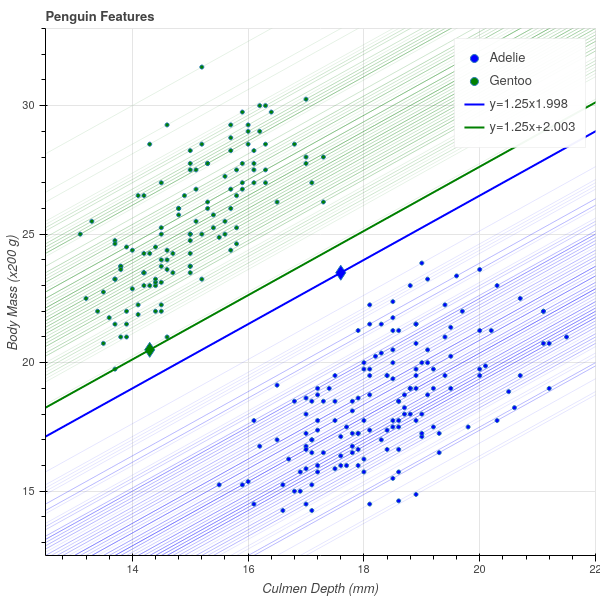
\includegraphics{../img/penguinhwy2.png}
\caption{Margin}
\end{figure}

\end{document}
